\documentclass{article}
\usepackage{graphicx} % Required for inserting images


\begin{document}

\begin{titlepage}
      \centering
      \vspace*{1cm}
    
     \Huge
     \textbf{Atividade 1 - Introdução à análise de dados em Física de Partículas}

     \vspace{0.5cm}
    
     \Large 
      Jully Moura Alves

     \vfill
    
     \Large
      Outubro de 2024
    \end{titlepage}

    \newpage
    \section*{Desenvolvimento}
    
    \vspace{0.5cm}

    Primeiro configuramos o computador:

    \vspace{0.5cm}

    \begin{figure}[hb]
        \centering
        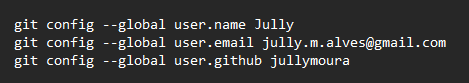
\includegraphics[width=1\linewidth]{global.png}
    \end{figure}

    \vspace{0.5cm}

    Depois criamos um repositório local:

    \vspace{0.5cm}

    \begin{figure}[hb]
        \centering
        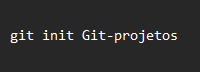
\includegraphics[width=0.4\linewidth]{init.png}
        \label{fig:enter-label}
    \end{figure}

    \vspace{0.5cm}

    Dentro deste repositório clonamos o repositório de Sheila:

    \vspace{0.5cm}
    
    \begin{figure}[hb]
        \centering
        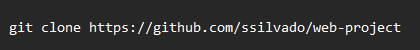
\includegraphics[width=0.9\linewidth]{clone.png}
        \label{fig:enter-label}
    \end{figure}

    \vspace{0.5cm}

    Logo após criamos uma nova branch: 

    \vspace{0.5cm}    

    \begin{figure}[!hb]
        \centering
        
\includegraphics[width=0.5\linewidth]{check.png}
        \label{fig:enter-label}
    \end{figure}

    \vspace{9cm}

    Em seguida utilizamos o comando abaixo para associar o repositório origin ao repositório indicado:

    \vspace{0.5cm}

    \begin{figure}[hb]
        \centering
        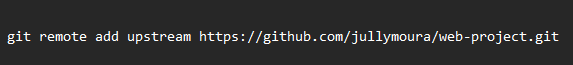
\includegraphics[width=1.2\linewidth]{remote.png}
        \label{fig:enter-label}
    \end{figure}

    \vspace{0.5cm}

    No passo seguinte, adicionamos uma linha de texto no final do arquivo arqteste.txt:

    \vspace{0.5cm}

    \begin{figure}[hb]
        \centering
        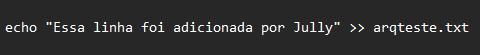
\includegraphics[width=1\linewidth]{echo.png}
        \label{fig:enter-label}
    \end{figure}

    \vspace{0.5cm}

    Com este comando conseguimos saber o estado atual do repositório:

    \vspace{0.5cm}

    \begin{figure}[hb]
        \centering
        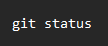
\includegraphics[width=0.25\linewidth]{status.png}
        \label{fig:enter-label}
    \end{figure}

    \vspace{0.5cm}

    Através do git add adicionamos alterações no seu repositório local à área de stage:

    \vspace{0.5cm}
    
    \begin{figure}[!hb]
        \centering
        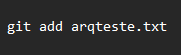
\includegraphics[width=0.4\linewidth]{add.png}
        \label{fig:enter-label}
    \end{figure}

    \vspace{9cm}

    Neste passo registramos as alterações feitas à área de stage. A opção -m permite que você inclua uma mensagem de commit diretamente na linha de comando descrevendo as mudanças que foram feitas. 

    \vspace{0.5cm}

    \begin{figure}[hb]
        \centering
        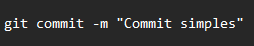
\includegraphics[width=0.55\linewidth]{commit.png}
        \label{fig:enter-label}
    \end{figure}

    \vspace{0.5cm}

    E, por fim, enviamos os commits locais para um repositório remoto e ligamos a branch local a branch remota:

    \vspace{0.5cm}

    \begin{figure}[hb]
        \centering
        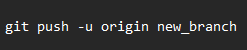
\includegraphics[width=0.55\linewidth]{push.png}
        \label{fig:enter-label}
    \end{figure}

    



\end{document}
